\titre{Resource :} Objet physique ou virtuel pouvant être alloué à un seul processus à la fois.\\

\titre{Resources retirables :} Peut être retirée au processus, utilisé par un autre, puis rendu au premier sans compromettre son exécution (exemples : CPU, RAM). \\

\titre{Resources non retirables :} Ne peut être retirée au processus que lorsqu'il en aura décidé. \\

\titre{3 étapes pour accéder à une resource non retirable :}
\begin{enumerate}
	\item Solliciter la resource
	\item Utiliser la resource
	\item Libérer la resource
\end{enumerate}

\titre{Famine :} Situation où un processus demande l'accès à une ressource mais ne l'obtient jamais car elle est toujours attribuée à d'autres processus.\\

\titre{Solution :} Le principe FIFO permet d'éviter la famine mais n'est pas toujours souhaitable. \\

\titre{Interblocage :} Situation où un ensemble de processus attendent un événement que seul un des processus de l'ensemble peut provoquer.\\

\titre{Exemple :}\\
\begin{tabular}{l|l}
Proc A & Proc B \\ \hline
Lock(M1) & Lock(M2) \\ 
Lock(M2) & Lock(M1) \\
\ldots & \ldots \\
Unlock(M2) & Unlock(M1) \\
Unlock(M1) & Unlock(M2) \\
\end{tabular}

\titre{Modélisation du problème : Modèle de Holt } (1972) On trace le graphe des attentes qui contient deux types de sommets (carré = ressource, rond = processus) \\
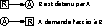
\includegraphics[width=100px]{fig37.pdf}\\

\titre{Exemple :}\\
\begin{tabular}{l|l|l}
A & B & C \\ \hline
D(R) & D(S) & D(T) \\
D(S) & D(T) & D(R) \\
L(R) & L(S) & L(T) \\
L(S) & L(T) & L(R) \\
\end{tabular} \\
Si l'ordonnancement est A,B,C,A,C on obtient : \\
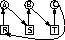
\includegraphics[width=100px]{fig38.pdf} \\

\titre{Stratégie face aux interblocages}
\begin{enumerate}
	\item Les ignorer
	\item Les détecter et y remédier 
	\begin{itemize}
		\item Mettre à jour dynamiquement le graphe des attentes lancer périodiquement un algo de détection des cycles. En cas d'interblocage on tue un des processus et on libère toutes ses ressources.
	\end{itemize}
	\item Détecter dynamiquement si il est sûr d'allouer une ressource
	\begin{itemize}
		\item 
		\begin{tabular}{l|l}
			A & B \\ \hline
			D(R) & D(S) \\
			D(S) & D(R) \\
			L(R) & L(S) \\
			L(S) & L(R) \\
		\end{tabular} \\
		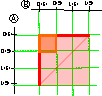
\includegraphics[width=100px]{fig39.pdf} \\
		On appelle état sûr un état à partir duquel on peut exécuter tous les processus un après l'autre dans un certain ordre sans qu'aucun ne soit bloqué. Un interblocage survient toujours à partir d'un état non sûr. \\ Pour déterminer les états sûrs, il faut connaitre à l'avance le code que vont exécuter les programmes. 
	\end{itemize}
	\item Imposer des contraintes pour s'assurer qu'un interblocage est impossible
	\begin{itemize}
		\item Pas d'exclusion mutuelle
		\item Ordonne les ressources
	\end{itemize}
\end{enumerate}
